
%% bare_conf.tex
%% V1.4b
%% 2015/08/26
%% by Michael Shell
%% See:
%% http://www.michaelshell.org/
%% for current contact information.
%%
%% This is a skeleton file demonstrating the use of IEEEtran.cls
%% (requires IEEEtran.cls version 1.8b or later) with an IEEE
%% conference paper.
%%
%% Support sites:
%% http://www.michaelshell.org/tex/ieeetran/
%% http://www.ctan.org/pkg/ieeetran
%% and
%% http://www.ieee.org/

%%*************************************************************************
%% Legal Notice:
%% This code is offered as-is without any warranty either expressed or
%% implied; without even the implied warranty of MERCHANTABILITY or
%% FITNESS FOR A PARTICULAR PURPOSE! 
%% User assumes all risk.
%% In no event shall the IEEE or any contributor to this code be liable for
%% any damages or losses, including, but not limited to, incidental,
%% consequential, or any other damages, resulting from the use or misuse
%% of any information contained here.
%%
%% All comments are the opinions of their respective authors and are not
%% necessarily endorsed by the IEEE.
%%
%% This work is distributed under the LaTeX Project Public License (LPPL)
%% ( http://www.latex-project.org/ ) version 1.3, and may be freely used,
%% distributed and modified. A copy of the LPPL, version 1.3, is included
%% in the base LaTeX documentation of all distributions of LaTeX released
%% 2003/12/01 or later.
%% Retain all contribution notices and credits.
%% ** Modified files should be clearly indicated as such, including  **
%% ** renaming them and changing author support contact information. **
%%*************************************************************************


% *** Authors should verify (and, if needed, correct) their LaTeX system  ***
% *** with the testflow diagnostic prior to trusting their LaTeX platform ***
% *** with production work. The IEEE's font choices and paper sizes can   ***
% *** trigger bugs that do not appear when using other class files.       ***                          ***
% The testflow support page is at:
% http://www.michaelshell.org/tex/testflow/



\documentclass[conference]{IEEEtran}
% Some Computer Society conferences also require the compsoc mode option,
% but others use the standard conference format.
%
% If IEEEtran.cls has not been installed into the LaTeX system files,
% manually specify the path to it like:
% \documentclass[conference]{../sty/IEEEtran}





% Some very useful LaTeX packages include:
% (uncomment the ones you want to load)


% *** MISC UTILITY PACKAGES ***
%
%\usepackage{ifpdf}
% Heiko Oberdiek's ifpdf.sty is very useful if you need conditional
% compilation based on whether the output is pdf or dvi.
% usage:
% \ifpdf
%   % pdf code
% \else
%   % dvi code
% \fi
% The latest version of ifpdf.sty can be obtained from:
% http://www.ctan.org/pkg/ifpdf
% Also, note that IEEEtran.cls V1.7 and later provides a builtin
% \ifCLASSINFOpdf conditional that works the same way.
% When switching from latex to pdflatex and vice-versa, the compiler may
% have to be run twice to clear warning/error messages.
\usepackage{textcomp}
\usepackage{booktabs}




% *** CITATION PACKAGES ***
%
%\usepackage{cite}
% cite.sty was written by Donald Arseneau
% V1.6 and later of IEEEtran pre-defines the format of the cite.sty package
% \cite{} output to follow that of the IEEE. Loading the cite package will
% result in citation numbers being automatically sorted and properly
% "compressed/ranged". e.g., [1], [9], [2], [7], [5], [6] without using
% cite.sty will become [1], [2], [5]--[7], [9] using cite.sty. cite.sty's
% \cite will automatically add leading space, if needed. Use cite.sty's
% noadjust option (cite.sty V3.8 and later) if you want to turn this off
% such as if a citation ever needs to be enclosed in parenthesis.
% cite.sty is already installed on most LaTeX systems. Be sure and use
% version 5.0 (2009-03-20) and later if using hyperref.sty.
% The latest version can be obtained at:
% http://www.ctan.org/pkg/cite
% The documentation is contained in the cite.sty file itself.

\usepackage[backend=bibtex,natbib=true]{biblatex}
\addbibresource{refs.bib}



% *** GRAPHICS RELATED PACKAGES ***
%
\ifCLASSINFOpdf
  % \usepackage[pdftex]{graphicx}
  % declare the path(s) where your graphic files are
  % \graphicspath{{../pdf/}{../jpeg/}}
  % and their extensions so you won't have to specify these with
  % every instance of \includegraphics
  % \DeclareGraphicsExtensions{.pdf,.jpeg,.png}
\else
  % or other class option (dvipsone, dvipdf, if not using dvips). graphicx
  % will default to the driver specified in the system graphics.cfg if no
  % driver is specified.
  % \usepackage[dvips]{graphicx}
  % declare the path(s) where your graphic files are
  % \graphicspath{{../eps/}}
  % and their extensions so you won't have to specify these with
  % every instance of \includegraphics
  % \DeclareGraphicsExtensions{.eps}
\fi
% graphicx was written by David Carlisle and Sebastian Rahtz. It is
% required if you want graphics, photos, etc. graphicx.sty is already
% installed on most LaTeX systems. The latest version and documentation
% can be obtained at: 
% http://www.ctan.org/pkg/graphicx
% Another good source of documentation is "Using Imported Graphics in
% LaTeX2e" by Keith Reckdahl which can be found at:
% http://www.ctan.org/pkg/epslatex
%
% latex, and pdflatex in dvi mode, support graphics in encapsulated
% postscript (.eps) format. pdflatex in pdf mode supports graphics
% in .pdf, .jpeg, .png and .mps (metapost) formats. Users should ensure
% that all non-photo figures use a vector format (.eps, .pdf, .mps) and
% not a bitmapped formats (.jpeg, .png). The IEEE frowns on bitmapped formats
% which can result in "jaggedy"/blurry rendering of lines and letters as
% well as large increases in file sizes.
%
% You can find documentation about the pdfTeX application at:
% http://www.tug.org/applications/pdftex

\usepackage{graphicx}



% *** MATH PACKAGES ***
%
%\usepackage{amsmath}
% A popular package from the American Mathematical Society that provides
% many useful and powerful commands for dealing with mathematics.
%
% Note that the amsmath package sets \interdisplaylinepenalty to 10000
% thus preventing page breaks from occurring within multiline equations. Use:
%\interdisplaylinepenalty=2500
% after loading amsmath to restore such page breaks as IEEEtran.cls normally
% does. amsmath.sty is already installed on most LaTeX systems. The latest
% version and documentation can be obtained at:
% http://www.ctan.org/pkg/amsmath





% *** SPECIALIZED LIST PACKAGES ***
%
%\usepackage{algorithmic}
% algorithmic.sty was written by Peter Williams and Rogerio Brito.
% This package provides an algorithmic environment fo describing algorithms.
% You can use the algorithmic environment in-text or within a figure
% environment to provide for a floating algorithm. Do NOT use the algorithm
% floating environment provided by algorithm.sty (by the same authors) or
% algorithm2e.sty (by Christophe Fiorio) as the IEEE does not use dedicated
% algorithm float types and packages that provide these will not provide
% correct IEEE style captions. The latest version and documentation of
% algorithmic.sty can be obtained at:
% http://www.ctan.org/pkg/algorithms
% Also of interest may be the (relatively newer and more customizable)
% algorithmicx.sty package by Szasz Janos:
% http://www.ctan.org/pkg/algorithmicx




% *** ALIGNMENT PACKAGES ***
%
%\usepackage{array}
% Frank Mittelbach's and David Carlisle's array.sty patches and improves
% the standard LaTeX2e array and tabular environments to provide better
% appearance and additional user controls. As the default LaTeX2e table
% generation code is lacking to the point of almost being broken with
% respect to the quality of the end results, all users are strongly
% advised to use an enhanced (at the very least that provided by array.sty)
% set of table tools. array.sty is already installed on most systems. The
% latest version and documentation can be obtained at:
% http://www.ctan.org/pkg/array


% IEEEtran contains the IEEEeqnarray family of commands that can be used to
% generate multiline equations as well as matrices, tables, etc., of high
% quality.
\usepackage{multirow}




% *** SUBFIGURE PACKAGES ***
%\ifCLASSOPTIONcompsoc
%  \usepackage[caption=false,font=normalsize,labelfont=sf,textfont=sf]{subfig}
%\else
%  \usepackage[caption=false,font=footnotesize]{subfig}
%\fi
% subfig.sty, written by Steven Douglas Cochran, is the modern replacement
% for subfigure.sty, the latter of which is no longer maintained and is
% incompatible with some LaTeX packages including fixltx2e. However,
% subfig.sty requires and automatically loads Axel Sommerfeldt's caption.sty
% which will override IEEEtran.cls' handling of captions and this will result
% in non-IEEE style figure/table captions. To prevent this problem, be sure
% and invoke subfig.sty's "caption=false" package option (available since
% subfig.sty version 1.3, 2005/06/28) as this is will preserve IEEEtran.cls
% handling of captions.
% Note that the Computer Society format requires a larger sans serif font
% than the serif footnote size font used in traditional IEEE formatting
% and thus the need to invoke different subfig.sty package options depending
% on whether compsoc mode has been enabled.
%
% The latest version and documentation of subfig.sty can be obtained at:
% http://www.ctan.org/pkg/subfig




% *** FLOAT PACKAGES ***
%
%\usepackage{fixltx2e}
% fixltx2e, the successor to the earlier fix2col.sty, was written by
% Frank Mittelbach and David Carlisle. This package corrects a few problems
% in the LaTeX2e kernel, the most notable of which is that in current
% LaTeX2e releases, the ordering of single and double column floats is not
% guaranteed to be preserved. Thus, an unpatched LaTeX2e can allow a
% single column figure to be placed prior to an earlier double column
% figure.
% Be aware that LaTeX2e kernels dated 2015 and later have fixltx2e.sty's
% corrections already built into the system in which case a warning will
% be issued if an attempt is made to load fixltx2e.sty as it is no longer
% needed.
% The latest version and documentation can be found at:
% http://www.ctan.org/pkg/fixltx2e


%\usepackage{stfloats}
% stfloats.sty was written by Sigitas Tolusis. This package gives LaTeX2e
% the ability to do double column floats at the bottom of the page as well
% as the top. (e.g., "\begin{figure*}[!b]" is not normally possible in
% LaTeX2e). It also provides a command:
%\fnbelowfloat
% to enable the placement of footnotes below bottom floats (the standard
% LaTeX2e kernel puts them above bottom floats). This is an invasive package
% which rewrites many portions of the LaTeX2e float routines. It may not work
% with other packages that modify the LaTeX2e float routines. The latest
% version and documentation can be obtained at:
% http://www.ctan.org/pkg/stfloats
% Do not use the stfloats baselinefloat ability as the IEEE does not allow
% \baselineskip to stretch. Authors submitting work to the IEEE should note
% that the IEEE rarely uses double column equations and that authors should try
% to avoid such use. Do not be tempted to use the cuted.sty or midfloat.sty
% packages (also by Sigitas Tolusis) as the IEEE does not format its papers in
% such ways.
% Do not attempt to use stfloats with fixltx2e as they are incompatible.
% Instead, use Morten Hogholm'a dblfloatfix which combines the features
% of both fixltx2e and stfloats:
%
% \usepackage{dblfloatfix}
% The latest version can be found at:
% http://www.ctan.org/pkg/dblfloatfix




% *** PDF, URL AND HYPERLINK PACKAGES ***
%
%\usepackage{url}
% url.sty was written by Donald Arseneau. It provides better support for
% handling and breaking URLs. url.sty is already installed on most LaTeX
% systems. The latest version and documentation can be obtained at:
% http://www.ctan.org/pkg/url
% Basically, \url{my_url_here}.




% *** Do not adjust lengths that control margins, column widths, etc. ***
% *** Do not use packages that alter fonts (such as pslatex).         ***
% There should be no need to do such things with IEEEtran.cls V1.6 and later.
% (Unless specifically asked to do so by the journal or conference you plan
% to submit to, of course. )


% correct bad hyphenation here
\hyphenation{op-tical net-works semi-conduc-tor}


\begin{document}
%
% paper title
% Titles are generally capitalized except for words such as a, an, and, as,
% at, but, by, for, in, nor, of, on, or, the, to and up, which are usually
% not capitalized unless they are the first or last word of the title.
% Linebreaks \\ can be used within to get better formatting as desired.
% Do not put math or special symbols in the title.
\title{A Position-Independent Method for Soil Types Recognition Using Inertial Data from a Wearable Device}

\author{
\IEEEauthorblockN{
	Florentin Thullier\IEEEauthorrefmark{1},
	Val\`ere Plantevin\IEEEauthorrefmark{1},
	Abdenour Bouzouane\IEEEauthorrefmark{1}, 
	Sylvain Hall\'e\IEEEauthorrefmark{2} and
	S\'ebastien Gaboury\IEEEauthorrefmark{1}
}

\IEEEauthorblockA{
	\IEEEauthorrefmark{1}LIARA Laboratory, Department of Computer Science and Mathematics, \\
	Universit\'e du Qu\'ebec \`a Chicoutimi, Chicoutimi, Qu\'ebec, Canada\\
	$Emails: \left\lbrace florentin.thullier1, valere.plantevin1, abdenour.bouzouane, sebastien.gaboury\right\rbrace@uqac.ca$
}
\IEEEauthorblockA{
	\IEEEauthorrefmark{2}LIF Laboratory, Department of Computer Science and Mathematics, \\
	Universit\'e du Qu\'ebec \`a Chicoutimi, Chicoutimi, Qu\'ebec, Canada\\
	$Email: shalle@uqac.ca$
}}

% make the title area
\maketitle

% As a general rule, do not put math, special symbols or citations
% in the abstract
\begin{abstract}
This paper describes a novel method for recognizing different soil types based on inertial data generated by a user's gait. To achieve this objective, a new wearable device which aims at collecting data produced by an embedded 6-axis accelerometer/gyroscope was designed first. To command this piece of hardware (start and stop recording, as well as annotate raw data), a mobile application was specifically developed. A total of 70 well-known features both from time and frequency domains that are mostly used in activity recognition were computed over each signal to produce enough discriminating characteristics. Then, two machine learning algorithms (Random Forest and $k$-Nearest Neighbors) were employed to classify such data. The proposed method was tested with 9 participants on four soil types with an experimental setup close to real use case situations. Results obtained let us state that a soil-types recognition is not only possible but also accurate and reliable since overall median F-Score measures of 82\% and 86\% were obtained respectively with the Random Forest and the $k$-NN classifiers. Although the user independence of our system was not proven due to a limited number of involved users, the independence condition of the position of the wearable device was clearly demonstrated.
\end{abstract}

\begin{IEEEkeywords}
Soil Types, Recognition, Wearable Object, IMU, Position-Independent
\end{IEEEkeywords}

% For peer review papers, you can put extra information on the cover
% page as needed:
% \ifCLASSOPTIONpeerreview
% \begin{center} \bfseries EDICS Category: 3-BBND \end{center}
% \fi
%
% For peerreview papers, this IEEEtran command inserts a page break and
% creates the second title. It will be ignored for other modes.
\IEEEpeerreviewmaketitle



\section{Introduction \& Related Work}
In the past few years, brand manufacturers have pushed the wearable 
technology in the forefront of the consumer electronics scene. As a result, in 2014, there was 15\% of mobile devices users employing a wearable device in their daily lives (\textit{e.g.} smartwatches or fitness band) \cite{Nielsen2014}. These devices have, first, brought more sensors than the ones already embedded in current smartphones. Moreover, the increasing use of the Bluetooth Low Energy (BLE) technology \cite{Taplett} allowed a more efficient communication with mobile devices as regards energy consumption. In that sense, wearable devices become widely adopted in order to track activities since they present a convenient and portable way to record physiological data produced by their users. Hence, a considerable amount of data is collected each day and several statistical analyses are offered for monitoring carriers' daily activities \cite{Patel2015}. Besides, according to recent advancements in machine learning, it is possible to say that existing activity tracking applications may be enhanced to become more ubiquitous (applications that aim to make devices more mobile and smart). Consequently, this research aims at answering three main hypotheses which may be summarized by the following question: \textit{"Is it possible to recognize soil types through inertial data produced by the human gait with a wearable device\textemdash whatever where it is positioned and by whom it is carried ?"}

The idea of recognizing soil-type, also known as terrain classification, through data produced by an accelerometer, comes from the mobile robotics area. First of all, \citet{Vail2004} experimented a surface detector using inertial data generated by a four-legged robot. Authors opted for a C4.5 decision tree since it is fast enough and simple to represent. In order to quantify the accuracy of their learning model, they used a 10-fold cross-validation method which gives us an overall accuracy of 84.9\% (cement: 91\%; carpet: 81.2\%; field: 81.2\%). 
 
Besides, \citet{Bibuli2007} suggested a terrain classification method for a four-wheels mobile robot equipped with several sensors, including inertial ones. The terrain classification was performed by providing frequency components of the signal, obtained through the Discrete Fourier Transform (DFT), as inputs of an artificial neural network (ANN). Moreover, since they trained one ANN by distinct axis, most valuable results were obtained with the training of the x-axis of the gyroscope, being respectively, 90\%, 71.2\%, 70\%, 98.8\% and 83.5\% for the gravel, grass, sand, pavement and dirt terrains.

In the same way, \citet{Weiss2007} proposed a comparison of terrain recognition for a four-wheeled robot between the Support Vector Machine (SVM) and several other classification techniques. Input data for the SVM algorithm were either a log-scaled Power Spectral Density, or a 128-point FFT features vector. Authors performed the experiment over different velocities of the robot (\textit{i.e.} 0.2, 0.4 and 0.6 m/s) and they obtained most accurate results with SVM rather than other algorithms, such as Probabilistic Neural Network (PNN), $k$-Nearest Neighbors ($k$-NN), Na\"ive Bayes and C4.5. 

Conversely, \citet{Kertesz2016} recently introduced a rigidity-based surface recognition for a four-legged robot using features extracted through the Fast Fourier Transform (FFT), then, classified with the Random Forest algorithm. The model was evaluated thanks to the 10-folds cross validation method. Authors found that the Random Forest outperformed every other algorithms it was compared to, as they obtained an accuracy of 96.2\%.

Although such a related literature was relevant in understanding how to answer hypotheses we formulated, all of these methods are not suitable for soil-types-recognition in a human walking context. Nevertheless, based on our current knowledge, we report a more recent study suggested by \citet{Otis2016} that introduced a terrain discrimination analysis to reduce the risk of falling through a three-axis accelerometer embedded in a shoe. A clustering algorithm was employed in order to segment FFT-based discriminating features. These characteristics were obtained from raw signals recorded on broken stone, concrete, sand, stone dust, snow and ice. As regards obtained results, authors reported a misidentification rate between 1\% and 5\% in the laboratory setup, while it rose up to 20\% in real conditions.

Furthermore, since it is known that human activity recognition performed thanks to accelerometers achieve excellent results \cite{Bayat2014, Bussmann2001, Cleland2013, Gao2014, Kwapisz2011, Ravi2005, Shoaib2013, Tuncel2009}, this work aims at combining these techniques with terrain discrimination methods reported above in order to recognize soil types based on the human gait.

The rest of the paper is structured as follows: section 2 details the suggested method for soil type recognition based on inertial data. Next, section 3 describes experiments we conducted in order to assess the three previously expressed hypotheses. Section 5 exposes and discusses results we obtained. Finally, section 6 draws a conclusion and section 7 provides future works.

\section{Proposed solution}

This section describes in details the proposed solution to verify the three assumptions that we have formulated in order to recognize soil types through inertial data. The first subsection explains the wearable device that we designed. Then, we present which discriminating features that are computed over raw data, then stored on such a piece of hardware. Finally, the last point of this section presents the two algorithms we have exploited to achieve the classification process.

\subsection{Hardware}

In order to test our approach and record several datasets, we designed a new wearable device which aims at receiving commands from a smartphone and saving a big amount of data produced by an Inertial Measurement Unit (IMU) as well. To satisfy these requirements, we decided to use the latest \textit{Intel Curie} board from \textit{Arduino} (a.k.a.\textit{ Arduino 101}) with a proto shield providing a SD card slot, as shown in Figure \ref{fig:arduino}. These choices were motivated by two main characteristics which are already present on the board. First of all, it is capable of communicating through Bluetooth Low Energy (BLE), a wireless technology embedded in many smartphones \cite{Taplett}, which offers a very low power consumption \cite{Gomez2012}. Secondly, the \textit{Intel Curie} offers a 6-axis accelerometer/gyroscope and enough Inputs/Outputs (I/O) to interface other hardware, for example, either an SD card for large storage or another IMU with more axis. 

\begin{figure}[!t]
  \centering
  \includegraphics[width=1.8in]{arduino_101}
  \caption{Arduino 101 board (1) and the dedicated proto shield with SD card slot (2).}
  \label{fig:arduino}
\end{figure}

The firmware \cite{Plantevin2016} embedded on the device is divided into three main components that are summed up in Figure \ref{fig:hardware}. The first one is the command module. It is in charge of all the communications between a mobile device and the hardware through the BLE radio module. Thereby, anyone using a phone (or any other device) that provides such a technology could set every mandatory parameters (\textit{i.e.} the type of soil, the participant's identification and the sensor location) before starting the recording. The second main component is the IMU  recorder. Its goal is to store in a buffer, values coming from the IMU over an SPI bus, at a stable frequency of 60 Hz. Finally, the buffer sends all its values in the dataset formatting module, every seconds. This component takes all the configuration parameters from the command module and creates formatted strings that are written on the memory card. 

\begin{figure}[!ht]
  \centering
  \includegraphics[width=3in]{hardware}
  \caption{Graphical representation of the firmware implementation embedded in the wearable device.}
  \label{fig:hardware}
\end{figure}

\subsection{Features Extraction}

Following the recording phase, where raw data produced by the IMU were saved on the memory of the device, a features extraction process must be achieved before classify them with machine learning algorithms. In that sense, we opted for 70 well-known features \cite{Bussmann2001, Bayat2014, Cleland2013, Kwapisz2011, Yang2008, Ravi2005, Shoaib2013, Gao2014}, that came from both time and frequency domains. They are all computed from a fixed non-overlapping time window over each raw signal.

On the first hand, the time-related ones are composed of 11 statistical computations. The first operation is a simple unweighted mean on each axis for each sensor (\textit{i.e.} gyroscope and accelerometer). Then, the average of these values for each specific sensor is processed. In the exact same way, we apply few more statistical calculations: the standard deviation, the \textit{skewness}, the \textit{kurtosis}, the \textit{Zero-crossing rate} and finally, the correlation between all possible axis combinations. Formulas of the $skewness$ and the $kutosis$ measures, when applied to the $X$ axis are respectively reminded in (\ref{eq:skewness}) and (\ref{eq:kurtosis}). In both cases, $N$ represents the number of elements in the vector, $x_i$ is the $i^{th}$ element in it, $\bar{X}$ is the mean of the vector and $\sigma_x$ refers to its standard deviation. Finally, we calculate the correlation between each axis combination from the same sensor as recalled by (\ref{eq:correlation}).

\begin{equation}
	\label{eq:skewness}
	skw(X) = \frac{N}{(N-1)(N-2)}\cdot\left(\sum_{i=1}^{N}{\frac{(x_i-\bar{X})^3}{\sigma_x^3}}\right)
\end{equation}

\begin{equation}
	\label{eq:kurtosis}
	\resizebox{.9\columnwidth}{!} 
	{
  		$kurtosis(X) = \frac{N(N+1)}{(N-1)(N-2)(N-3)}\cdot\left(\sum_{i=1}^{N}{\frac{(x_i-\bar{X})^4}{\sigma_x^4}-\frac{3(N-1)^2}{(N-2)(N-3)}}\right)$
  	}
\end{equation}

\begin{equation}
	\label{eq:correlation}
	\rho(X,Y) = \frac{cov(X,Y)}{\sigma_x\cdot\sigma_y}
\end{equation}

On the second hand, several attributes required to be transformed from the time domain to the frequency one. In order to achieve such a conversion, the Fast Fourier Transform (FFT) algorithm has been used. These three features are the DC component, the Entropy of each axis frequency representation and finally, the Energy that is defined in (\ref{eq:energy}), where $X$ represent a vector of complex numbers, $N$ refers to its size and $x_i$ is the $i^{th}$ element in it.

\begin{equation}
	\label{eq:energy}
	Energy(X) = \frac{1}{N}\cdot\left(\sum_{i=1}^{N}|x_i|\right)
\end{equation}

\subsection{Classification}

Once discriminating features extracted from raw inertial data are computed, the following task that must be achieved by our system is a classification process. According to the literature in the field of activity recognition, as well as terrain classification in robotics, it is known that several of such algorithms achieve excellent results in classifying data from inertial sensors. As examples, we can mention: Decision Trees (DT), $k$-Nearest Neighbors ($k$-NN), Support Vector Machines (SVM), Artificial Neural Networks (ANN), and Na\"ive Bayes \cite{Tuncel2009, Kertesz2016, Weiss2007, Kim2010, Vail2004, Hoffmann2014, Bibuli2007}. 

In that sense, this research exposes a direct comparison between the Random Forest and the $k$-Nearest Neighbors algorithms when applied on soil type recognition. We justify such a choice, first because they belong to two distinct families of classifiers\textemdash respectively, the decision trees and the lazy learning ones. Moreover, as non-parametric methods (methods that do not make strong assumptions about the form of the mapping function), these algorithms remains simple, flexible, powerful and efficient \cite{Russell2010}. Indeed, their satisfying classification performance is, most of the time, reported in the literature \cite{Kertesz2016, Vail2004}.

\subsubsection{Random Forest}

According to \citet{Breiman2001}, a Random Forest (RF) is a combination of tree predictors, where each tree depends on the values of a random vector, sampled independently and with the same distribution for all trees in the forest. The final decision is made by a majority vote between each outcome of each single tree that forms the forest. Figure \ref{fig:rf} exposes a simple example of a Random Forest classification using three trees. Such a classification algorithm implies several initial parameters. The three most important ones which are necessary to define are first, the number of trees in the forest ($B$), second, the number of features to consider when looking for the best split ($F$) and the function used to measure the quality of such a split ($C$). According to the literature, \citet{Breiman2001} suggests using $F=log_2(m) + 1$ where $m$ refers to the number of attributes present in the dataset. However, it is also possible to find other recommendations such as $F=\frac{1}{2}\sqrt{m}$ or $F=\sqrt{m}$. As regards the quality of the split, the two primary function often employed are first, the calculation of the Gini index and second, the evaluation of the information gain that are respectively expressed by (\ref{eq:gini}) and (\ref{eq:gain}):

\begin{equation}
	\label{eq:gini}
	Gini(T) = {1-\sum_{i=1}^{n}(p_i)}^2
\end{equation}

\begin{equation}
	\label{eq:gain}
	E(T) = \sum_{i=1}^{n}-(p_i log_2 p_i)
\end{equation}

\noindent where $T$ are input data containing instances of $n$ classes and $p_i$ is the relative frequency of class $i \in n$ in $T$. However, this criterion depends essentially of the type of trees that are used in the construction of the forest (\textit{i.e.} ID3, C4.5, CART, \textit{etc.}).

\begin{figure}[!t]
  \centering
  \includegraphics[width=3in]{rf}
  \caption{A simple example of a Random Forest classification using $B = 3$ trees.}
  \label{fig:rf}
\end{figure}

\subsubsection{$k$-Nearest Neighbors}

Firstly, this algorithm is a non parametric classification algorithm. In other words, it does not make any assumption on the underlying data distribution. Moreover, it is a lazy algorithm which means that there is no training phase, or it is very minimal. Although $k$-NN is a very fast algorithm, the final classification decision is made based on the entire training dataset that necessarily involve to have some storage space. Indeed, it assumes that the data are in a feature space since they may be scalars or multidimensional vectors. The $k$ closest vectors are extracted by using a distance measure and classes of new unknown data are defined through a majority vote between the label of each class of these $k$ neighbors. Figure \ref{fig:knn} shows a simple example of such a classification when $k=3$ nearest neighbors.

\begin{figure}[!t]
  \centering
  \includegraphics[width=3in]{knn}
  \caption{A simple example of a 3-Nearest Neighbors classification.}
  \label{fig:knn}
\end{figure}

Once the parameter $k$ is set, it is also important to select the proper distance measure to use for obtaining the $k$ closest vectors. Here, we describe two well-known distance measures: the Euclidean (\ref{eq:d_eucl}) and the Manhattan (\ref{eq:d_manh}) ones. 

\begin{equation}
	\label{eq:d_eucl}
	D_{Euclidean} = \sqrt{\sum_{i=1}^{n}(x_i-y_i)^2}
\end{equation}

\begin{equation}
	\label{eq:d_manh}
	D_{Manhattan} = \sum_{i=1}^{n}\left|x_i-y_i\right|
\end{equation}

\section{Experiments}

Experiments we have conducted involved, first of all, several participants that are described in the first point of this section. Moreover, both the requirements of the experiment and the procedure of the data collection are described in the two following subsections. 

\subsection{Participants}

We recruited 9 university students as participants. They were all males from 22 to 36 years old. Their weights were placed between 65 kg and 110 kg (median: 80 kg), and their heights were between 172 cm and 192 cm (median: 183 cm) respectively. Moreover, we counted up 7 right-handed persons and 2 left-handers. All of them were healthy people without any motor function issues.

\subsection{Requirements}

The experiment we have conducted involve several requirements. 

On the first hand, since our University is located in a region with hard weather conditions, most of the different soil types are recovered either, or both, of ice or snow. To cope with such an issue, we have built a box which was filled with few of the most common soil types that is possible to find outside (\textit{i.e.} gravel and sand). The box was 215 cm long and 90 cm wide as shown on Figure \ref{fig:box}.

\begin{figure}[!t]
  \centering
  \includegraphics[width=2in]{box}
  \caption{The box used for our experiments filled first with gravel and then with sand.}
  \label{fig:box}
\end{figure}

On the second hand, we needed to tell the wearable device when to start and stop, and how to annotate correctly each record. To this end, we have developed an \textit{Android} application \cite{Thullier2016b} that was run on a \textit{LG Nexus 5} with the 6.0.1 version of \textit{Android}. The main benefit of such an application is the mobility allowed by the smartphone instead of a traditional desktop computer application. Since the wearable device provide a Bluetooth Low Energy (BLE) connectivity, the first task to perform with the application is to scan all the devices available in this network and to pair with ours through the application, as exposed in the first screen of the Figure \ref{fig:android_app}. Then, the second screen shows the interface that allowed us to annotate each record with the following information: the soil type on which the user is about to walk, the position of the wearable device (within: \textit{backpack}, \textit{left} and \textit{right hand bag}, and \textit{left} and \textit{right pocket}), as well as the identification of the current participant (where each one was anonymized by a capital letter).

\begin{figure}[!t]
  \centering
  \includegraphics[width=3in]{android_app}
  \caption{Screens of the Android application which was used to pair with the device and pilot the annotation of the inertial data records.}
  \label{fig:android_app}
\end{figure}

\subsection{Procedure}

To perform the data collection, we attempted to get as close as possible to real use case situations. 

In that sense, we judge that the three most natural places where a user may wear the device are: a hand-bag, a backpack and inside the pocket of a jacket. However, since we wanted to determine the impact of the location of the device accurately, participants were asked to wear the device both on the right and left shoulders for the hand-bag, as shown in Figure \ref{fig:positions_hand_bags}. Moreover, such a bag was ballasted with an extra weight of 1 kg. In the same way, participants were requested, to wear the device both inside the right and left pockets of the jacket, as illustrated in the left of Figure \ref{fig:positions}, where a special attention was placed on keeping the jacket closed. We have formulated such a requirement in order to reduce variable noise that may have been created on inertial data because of the proper arm balancing of each participant. Finally, the last position we have experienced here, concerns the positioning inside a standard 20 L hiking backpack which weighed approximately 3 kg. The device was placed in both the same pocket and direction for each participant as demonstrated in the right of Figure \ref{fig:positions}

\begin{figure}[!t]
  \centering
  \includegraphics[width=3.25in]{positions_hand_bags}
  \caption{Position of the wearable device inside the hand bag being both on the left and the right shoulder.}
  \label{fig:positions_hand_bags}
\end{figure}

\begin{figure}[!b]
  \centering
  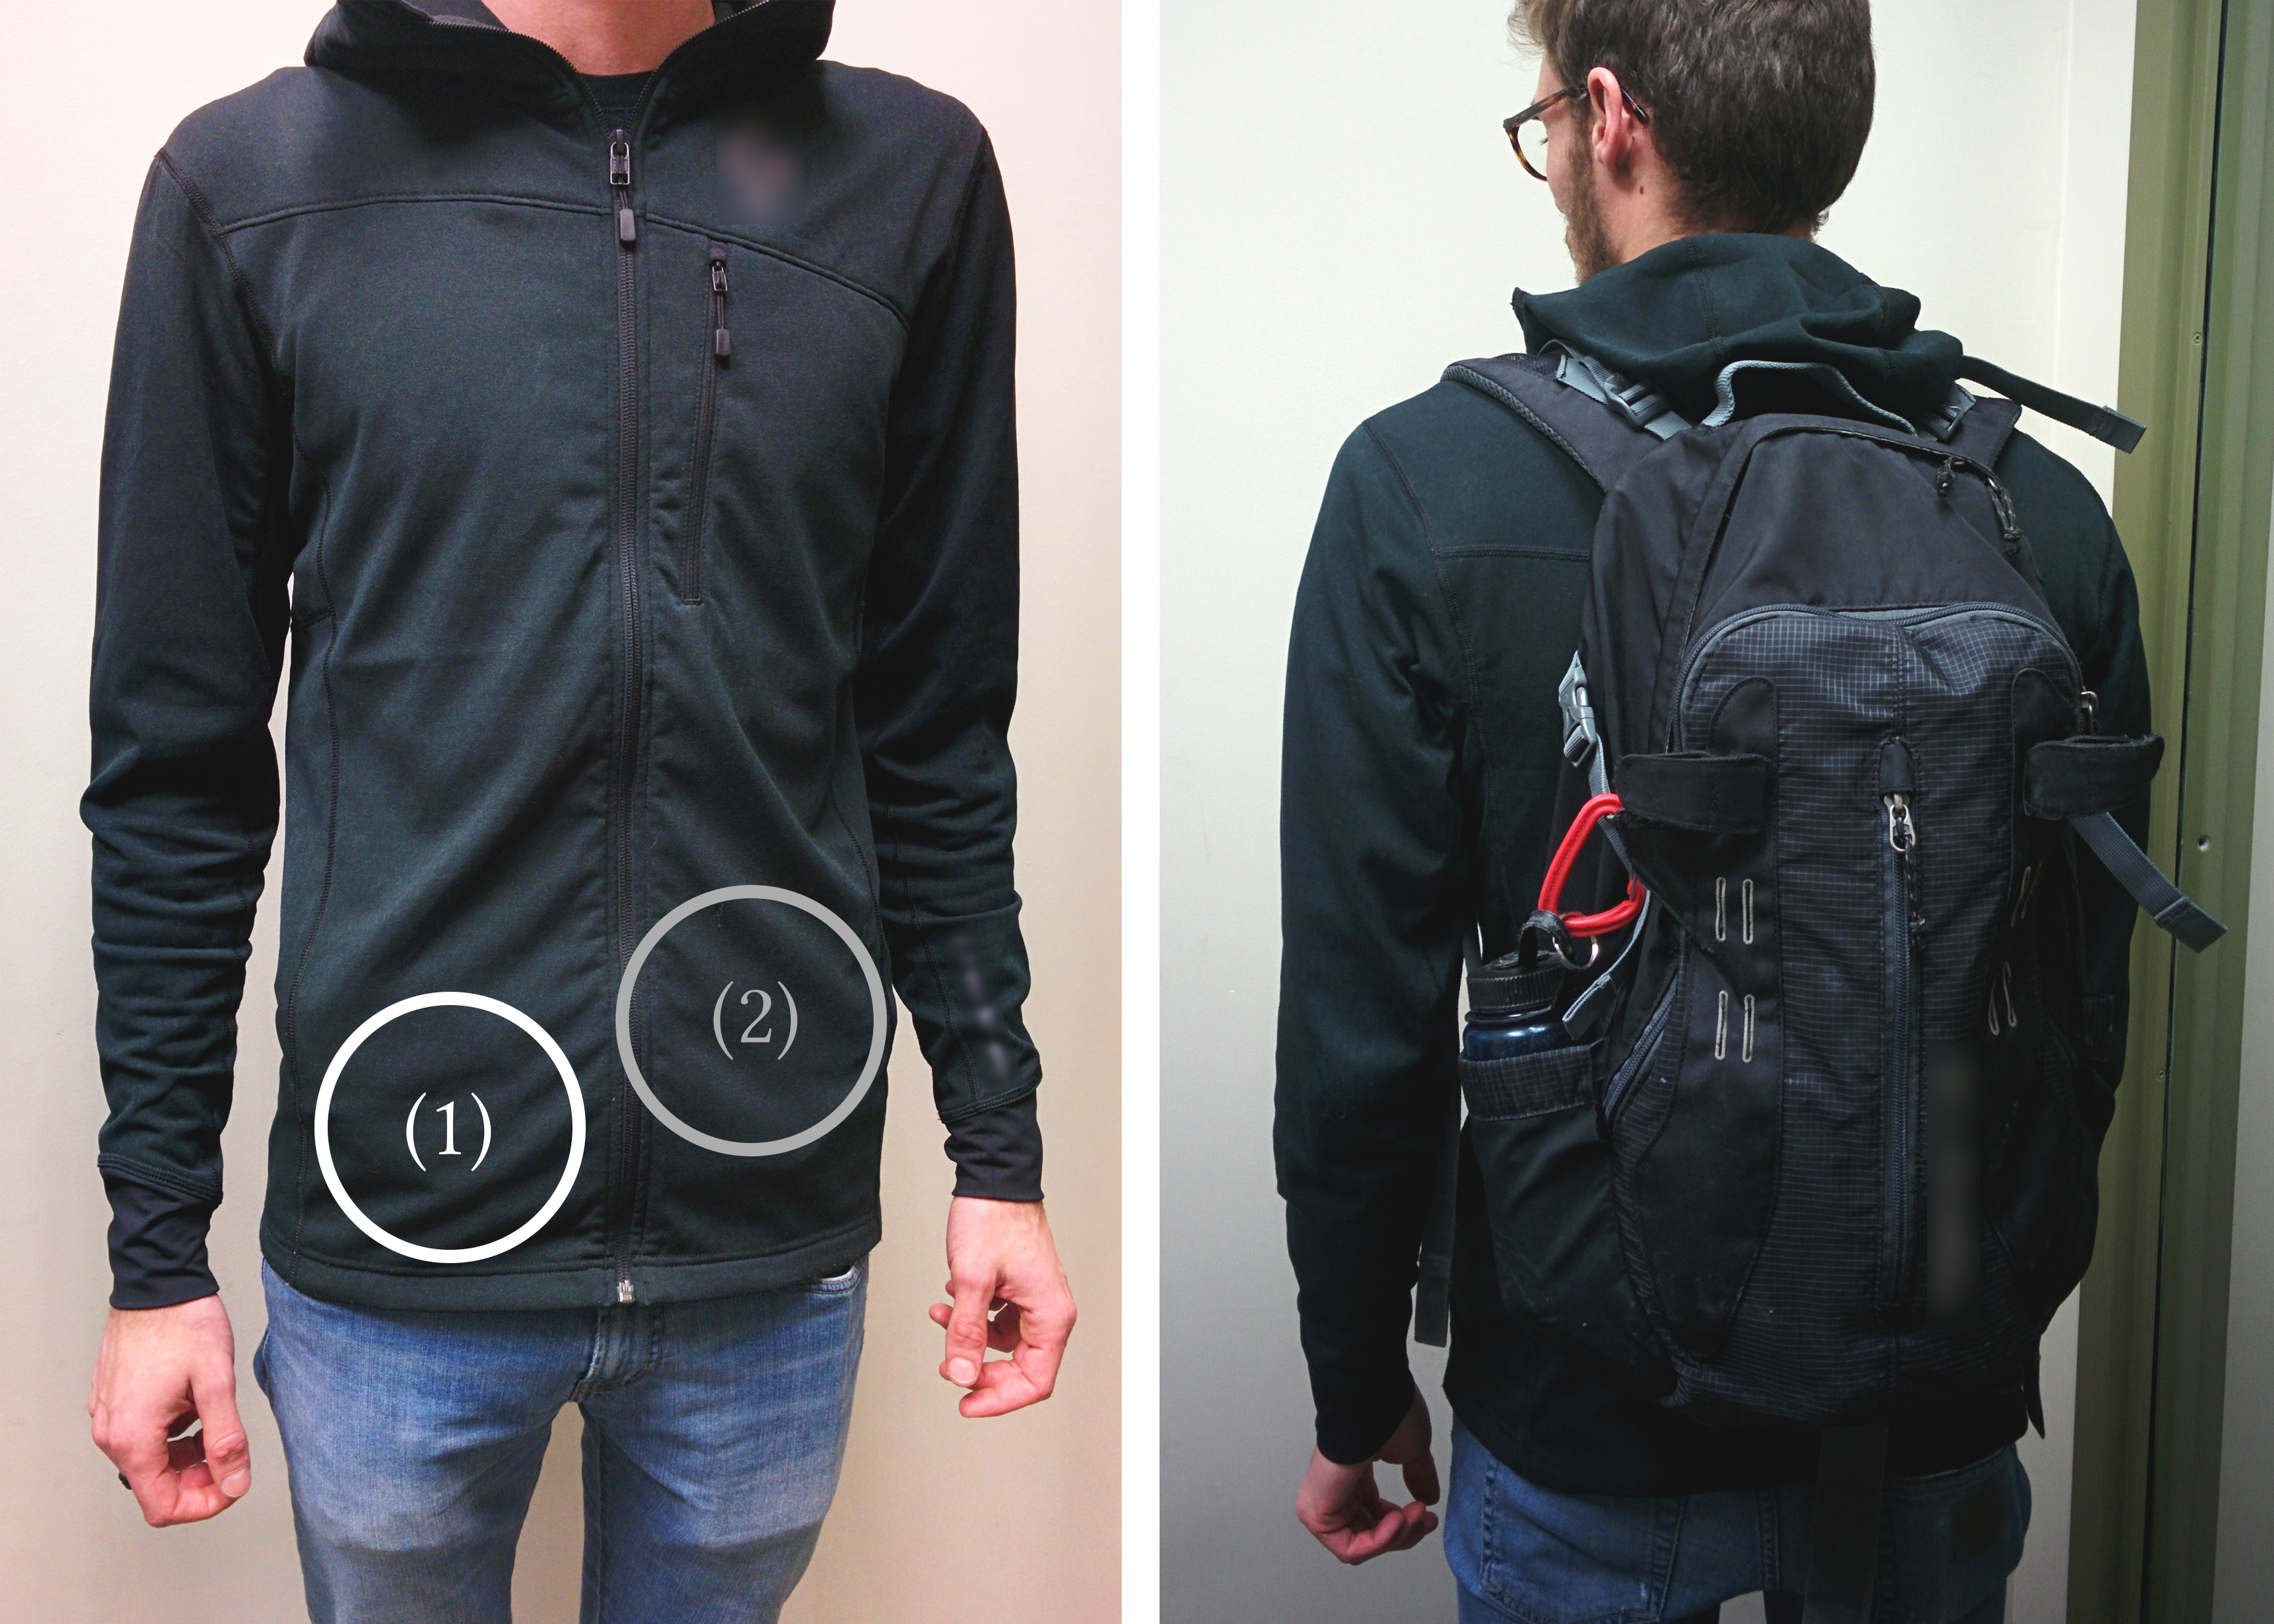
\includegraphics[width=3.25in]{positions}
  \caption{From left to right, position of the wearable device inside both right (1) and left (2) front jacket pockets and inside a standard 20L backpack.}
  \label{fig:positions}
\end{figure}

Once participants were introduced how to wear the device, they were invited to perform six round trips on each soil types, for each given position. A supervisor, in charge of the management of the device through the \textit{Android} application, let them know both when to start and stop walking. Firstly, they were asked to begin by gravels that were placed inside the box described previously. Secondly they were requested to perform the same operation on the floor next to the container that is considered to be a kind of cement. Then, we have invited participants to go outside to perform another six round trip in the snow. In order to remain consistent with the characteristics of records we collected inside, a measuring tape\textemdash respecting the length of the box\textemdash was placed over the snow to inform participants where to turn around. Finally, since we needed to replace gravels inside the container, participants were called back\textemdash at another stage\textemdash to perform the experiment once more, on the sand.

\section{Results and discussion}

\subsection{Classification Performance Metrics}

Since the performance of the classification task requires to be properly evaluated, it is important to provide representative metrics. 

To this end, the accuracy ($Acc.$) is probably the most dominant measure in the literature because of its simplicity. This measure provides the ratio between the correct number of predictions and the total number of cases given as,

\begin{equation}
	\label{eq:f_acc}
	Acc. = \frac{TP + TN}{TP + TN + FP + FN}
\end{equation}

\noindent where $TP$ and $TN$ refer to true positive and true negative predictions respectively, and the total additionally include false positive ($FP$) and false negative ($FN$) predictions.

Despite its popularity, accuracy alone does typically not provide enough information to evaluate the robustness of prediction outcomes. Indeed, accuracy does not compensate for results that may be expected by luck. Indeed, a high accuracy does not necessarily reflect an indicator of a high classification performance. This is the accuracy paradox. For instance, in a predictive classification setting, predictive models with a given level of accuracy may have greater predictive power than models with higher accuracy. In that sense, as suggested by \citet{Ben-David2007}, we decided to provide the Cohen\textquotesingle s kappa ($k$) evaluation metric as well. This measure takes into account such a paradox and remains a more relevant metric in classification evaluation such as the method we suggest in this paper. The kappa measure is given by,

\begin{equation}
	\label{eq:kappa}
	k = \frac{P_o-P_e}{1-P_e}
\end{equation}

\noindent where $P_o$ and $P_e$ are the observed and the expected probabilities respectively. 

Another well-known metrics which is often used in related literature and which we choose to provide additionally,  is the F-Score,

\begin{equation}
	\label{eq:f_score}
	F-Score = 2\cdot\frac{Precision . Recall}{Precision + Recall}
\end{equation}

\noindent $Precision$ and $Recall$ are expressed by (\ref{eq:precision}) and (\ref{eq:recall}) respectively,

\begin{equation}
	\label{eq:precision}
	Precision = \frac{TP}{TP + FP}
\end{equation}

\begin{equation}
	\label{eq:recall}
	Recall = \frac{TP}{TP + FN}
\end{equation}

\noindent where $FP$ and $FN$ refer to false positive and false negative predictions respectively and $TP$ corresponds to true positive results.

\subsection{Datasets}

Once every participant has achieved the experiment on all soil types, we had to produce several datasets in order to make sure that the method we suggest in this paper was accurate and reliable enough. Details about each dataset are provided in Table \ref{tab:datasets}, and they were all made freely accessible to the public \cite{Thullier2017}. 

As we have detailed in above section, the data sampling provided by our wearable device was made at a 60 Hz frequency. Moreover, we have observed an average time of 6 seconds for participants to complete a round trip both inside, in the box, as well as outside. Hence, we have decided to split our dataset in several subsets of $6 \times 60$ instances in order to produce one sample per round trip. Thus, we obtained a total of 5 samples, for each participant, on each soil type, for each position of the device on which features were extracted.

\begin{table}[!ht]
    \centering
    \caption{The detailed list of datasets we have produced through our experiment.}
    \label{tab:datasets}
    \begin{tabular}{rl}
    	\toprule
        \textbf{Dataset}&\textbf{Description}\\
        \midrule
    	\multirow{2}{*}{Soil types}&Instances are annotated\\&only with the related soil type.\\
    	\midrule    	
    	\multirow{3}{*}{Soil type given participant}&Instances are annotated both\\&with the related soil type and the\\&participant's letter.\\
    	\midrule  
    	\multirow{3}{*}{Soil type given position}&Instances are annotated both\\&with the related soil type and the\\&location of the wearable device.\\
    	\bottomrule
    \end{tabular}
\end{table}

Since it is known that the human gait is considered to be a behavioral biometric \cite{Thullier2016c}, we have constructed one particular dataset containing each soil type for each participant of our experiment. Hence, these 9 datasets let us experiment the user-independent assumption of our method. Moreover, since we have exploited several positions for the wearable device, we have also created one dataset containing every soil types for each given place, being 5 distinct datasets in total. In that sense, we have been able to test the position-independent hypothesis as well. 

\subsection{Results Obtained}

The performance of the proposed method for soil types recognition was evaluated according to several classification analyses. These assessments were achieved thanks to the \textit{WEKA} datamining software \cite{Hall2009} which was used as a library in a simple open-source \textit{Java} Command Line Interface (CLI) application \cite{Thullier2016a}. Through this program, a 10-folds cross validation method was employed to quantify each trained model that was constructed. 


First of all, we aimed at verifying the first assumption by creating few Random Forest models based on several parameters tuning. Since it is preferable to have a great number of trees in the forest \cite{Breiman2001}, we have decided to experiment both 150 and 300 trees in order to preserve an acceptable computation time. Since a total of 70 discriminating attributes were obtained at the end of the features extraction process, the number of random variables ($F$) for the Random Forest was set to $F=\lfloor\frac{1}{2}\sqrt{70}\rfloor=4$, $F=\lfloor\log_2(70)+1\rfloor=7$ and $F=\lfloor\sqrt{70}\rfloor=8$. Finally, the default function used to measure the quality of the split which is implemented in \textit{WEKA} is the information gain. Results we have obtained for all of these layouts, given each dataset, are exposed in both Table \ref{tab:results_150} and \ref{tab:results_300}.

\begin{table}[!ht]
  \centering
  \caption{Results obtained with Random Forest classifier using 150 trees and from up to down: 4, 7 and 8 features as parameters for our three datasets.}
  \label{tab:results_150}
  \begin{tabular}{rccc}
    \toprule
    \textbf{Dataset}&\textbf{Acc.}&\textbf{F-Score}&\textbf{k}\\
    \midrule
   	Soil types&0.82&0.82&0.76\\
    Soil type given participant&0.78&0.78&0.77\\
    Soil type given position&0.86&0.86&0.85\\
\end{tabular}
\begin{tabular}{rccc}
    \toprule
    \textbf{Dataset}&\textbf{Acc.}&\textbf{F-Score}&\textbf{k}\\
    \midrule
   	Soil types&0.82&0.81&0.75\\
    Soil type given participant&0.77&0.77&0.77\\
    Soil type given position&0.87&0.87&0.86\\
\end{tabular}
\begin{tabular}{rccc}
    \toprule
    \textbf{Dataset}&\textbf{Acc.}&\textbf{F-Score}&\textbf{k}\\
    \midrule
   	Soil types&0.82&0.82&0.76\\
    Soil type given participant&0.77&0.76&0.76\\
    Soil type given position&0.87&0.87&0.86\\
  \bottomrule
\end{tabular}
\end{table}

\begin{table}[!ht]
  \centering
  \caption{Results obtained with Random Forest classifier using 300 trees and from up to down: 4, 7 and 8 features as parameters for our three datasets.}
  \label{tab:results_300}
  \begin{tabular}{rccc}
    \toprule
    \textbf{Dataset}&\textbf{Acc.}&\textbf{F-Score}&\textbf{k}\\
    \midrule
   	Soil types&0.87&0.83&0.77\\
    Soil type given participant&0.78&0.77&0.77\\
    Soil type given position&0.88&0.87&0.87\\
\end{tabular}
\begin{tabular}{rccc}
    \toprule
    \textbf{Dataset}&\textbf{Acc.}&\textbf{F-Score}&\textbf{k}\\
    \midrule
   	Soil types&0.84&0.84&0.78\\
    Soil type given participant&0.78&0.77&0.77\\
    Soil type given position&0.87&0.87&0.86\\
\end{tabular}
\begin{tabular}{rccc}
    \toprule
    \textbf{Dataset}&\textbf{Acc.}&\textbf{F-Score}&\textbf{k}\\
    \midrule
   	Soil types&0.82&0.82&0.76\\
    Soil type given participant&0.77&0.78&0.77\\
    Soil type given position&0.87&0.87&0.86\\
  \bottomrule
\end{tabular}
\end{table}

As regards such results, it is possible for us to state that the fitting parameters for our soil-types-recognition method when using a Random Forest are: 300 trees and a number of random attributes equivalent to $\log_2(m) + 1$. Indeed when considering this setup, the mean and the median F-Score measures correspond to the highest values observed for the overall results of this evaluation, being respectively, $84\%$ and $83\%$. 

Moreover, Table \ref{tab:conf_mat} exposes, in detail, the outcomes of the Random Forest classification using such recommended parameters over the \textquotedblleft\textit{soil types}" dataset. While a satisfactory overall classification performance was obtained with this setup, such a resulting confusion matrix let us discover that inertial data recorded on the \textit{cement} were the least well recognized within every soil types. Indeed these instances were, most of the time, mistakenly identified as \textit{gravel}. In the same way, the \textit{sand} was successfully recognized since only 17 instances were misidentified.

\begin{table}[!ht]
  \centering
  \caption{Resulting confusion matrix for the classification of instances from different soil types using recommended Random Forest parameters (\textit{i.e.} 300 trees, 7 features).}
  \label{tab:conf_mat}
  \begin{tabular}{cccccc}
    \toprule
    &\textbf{Cement}&\textbf{Gravel}&\textbf{Snow}&\textbf{Sand}\\
    \midrule
   	\textbf{Cement}&143&18&15&7\\
    \textbf{Gravel}&23&141&8&6\\
    \textbf{Snow}&2&2&208&4\\
    \textbf{Sand}&10&9&20&153\\
    \bottomrule
\end{tabular}
\end{table}

%\begin{figure}[!b]
%  \centering
%  \includegraphics[width=3.25in]{cement_results}
%  \caption{Classification results for instances of cement using recommended Random %Forest parameters (\textit{i.e.} 300 trees, 7 features).}
%  \label{fig:cement_results}
%\end{figure}

%\begin{figure}[!t]
%  \centering
%  \includegraphics[width=3.25in]{gravel_results}
%  \caption{Classification results for instances of gravel using recommended Random %Forest parameters (\textit{i.e.} 300 trees, 7 features).}
%  \label{fig:gravel_results}
%\end{figure}

%\begin{figure}[!t]
%  \centering
%  \includegraphics[width=3.25in]{snow_results}
%  \caption{Classification results for instances of snow using recommended Random %Forest parameters (\textit{i.e.} 300 trees, 7 features).}
%  \label{fig:snow_results}
%\end{figure}

%\begin{figure}[!t]
%  \centering
%  \includegraphics[width=3.25in]{sand_results}
%  \caption{Classification results for instances of sand using recommended Random %Forest parameters (\textit{i.e.} 300 trees, 7 features).}
%  \label{fig:sand_results}
%\end{figure}

Similarly, the performance of the $k$-Nearest Neighbors algorithm was evaluated over our three datasets, in order to compare the performance obtained with the Random Forest algorithm. The two measures of distance described previously were experienced in this appraisal and we found that the fitting number of neighbors to consider was only one. Indeed, all values from $k=1$ to $k=\sqrt{70}$ were tested and results were compared in an empirical manner to find such an optimal setting. Table \ref{tab:results_knn} only report a comparison of results that were obtained through a linear search of the nearest neighbor both with the Euclidean and the Manhattan distance measures.

\begin{table}[!ht]
  \centering
  \caption{Results obtained with K-Nearest Neighbor classifier (where $k=1$), using from up to down: the Euclidean and the Manhattan distance for our three datasets.}
  \label{tab:results_knn}
  \begin{tabular}{rccc}
    \toprule
    \textbf{Dataset}&\textbf{Acc.}&\textbf{F-Score}&\textbf{k}\\
    \midrule
   	Soil types&0.85&0.85&0.80\\
    Soil type given participant&0.79&0.78&0.78\\
    Soil type given position&0.83&0.83&0.82\\
\end{tabular}
\begin{tabular}{rccc}
    \toprule
    \textbf{Dataset}&\textbf{Acc.}&\textbf{F-Score}&\textbf{k}\\
    \midrule
   	Soil types&0.87&0.87&0.83\\
    Soil type given participant&0.80&0.80&0.80\\
    Soil type given position&0.85&0.85&0.84\\
  \bottomrule
\end{tabular}
\end{table}

Based on such results, we have observed that the classification performance, with the two distance measures, was analog to the ones that were achieved with the Random Forest algorithm, when tuned with our recommended parameters. However, we have noticed slightly superior results with the Manhattan distance measure comparatively to the Euclidean one. In that sense, regardless of these examinations, we state that parameters that must be applied, when using a $k$-NN to recognize soil types based on inertial data produced by human gait are: 1 nearest neighbor using the Manhattan distance.

Secondly, in order to validate the position-independent assumption, raw inertial data were separated by position and labeled, in agreement, with the corresponding soil type. Thus, five distinct datasets were produced, and they were evaluated both with the Random Forest and the $k$-NN algorithms respectively tuned with our previously suggested parameters. Results are shown in Figures \ref{fig:position_independent_rf} and \ref{fig:position_independent_knn}. The evaluation metric used as the position-independent baseline is the kappa measure, where 86\% and 84\% were respectively obtained for the Random Forest and the $k$-NN classifications over the \textquotedblleft\textit{soil type given position}" dataset.

\begin{figure}[!b]
  \centering
  \includegraphics[width=3.25in]{position_independent_rf}
  \caption{Kappa and F-Score measures comparison for both dependent and independent positions with Random Forest training, where 1: \textit{backpack}; 2: \textit{left hand-bag}; 3: \textit{left pocket}; 4: \textit{right hand-bag} and 5: \textit{right pocket}.}
  \label{fig:position_independent_rf}
\end{figure}

\begin{figure}[!t]
  \centering
  \includegraphics[width=3.25in]{position_independent_knn}
  \caption{Kappa and F-Score measures comparison for both dependent and independent positions with $k$-NN training, where 1: \textit{backpack}; 2: \textit{left hand-bag}; 3: \textit{left pocket}; 4: \textit{right hand-bag} and 5: \textit{right pocket}.}
  \label{fig:position_independent_knn}
\end{figure}

Although preceding overall results were indeed accurate, it is possible to observe an excellent performance when the learning process is achieved separately for each position as well. Indeed, when the Random Forest algorithm is used, there is no specific position greater than the baseline value (\textit{i.e.} 86\%) and the fourth positions which are above the baseline (\textit{i.e.} 84\%) with the $k$-NN algorithm yet remain really close to such a value.

Finally, the last experiment we proceed in this research refers to the user-independent hypothesis. In the same way as the position-independent assessment, eight datasets were generated (one by participant) and annotated, accordingly, with the corresponding soil type. Figure \ref{fig:user_independent_rf} and \ref{fig:user_independent_knn} expose obtained results, where the first chart is the Random Forest model and the second corresponds to the $k$-NN one. Both of them were computed with the same parameters as the previous analysis.

\begin{figure}[!t]
  \centering
  \includegraphics[width=3.25in]{user_independent_rf}
  \caption{Kappa and F-Score measures comparison for both dependent and independent users with Random Forest training, where each letter refers to a given participant.}
  \label{fig:user_independent_rf}
\end{figure}

\begin{figure}[!t]
  \includegraphics[width=3.25in]{user_independent_knn}
  \caption{Kappa and F-Score measures comparison for both dependent and independent users with $k$-NN training, where each letter refers to a given participant.}
  \label{fig:user_independent_knn}
\end{figure}

Yet again, when compared to results that were achieved in the past experiment, the performance we have obtained when learning each participant individually with both algorithms remains excellent. However, there are more than half of given sets where the kappa measure exceeds the baseline value (\textit{i.e.} respectively 77\% and 80\%, with the Random Forest and the $k$-NN algorithms). Hence, according to such a small number of participants, it is impossible for us to state that our proposed soil-types-recognition method is user-independent. 

\subsection{Discussion}

In this research, we have ventured three main hypotheses. The first one was referring to the possibility of recognizing several soil types through inertial data produced by the human gait. According to results exposed in the previous section, it is possible for us to say that such a recognition is fully achievable. Indeed, when it was a matter of classifying only soil types, we have obtained a classification accuracy of 82\% in the worst case. Although such a performance remains excellent, we have obtained a maximum accuracy of  87\% on the same dataset, with both the Random Forest and the $k$-NN algorithms tuned with parameters that we assessed as the most suitable for this problem.

Then, following assumptions expressed in this work were the user and the position independency conditions. Experiments we have conducted to validate these two hypotheses both outcome an excellent classification performance in the learning processes, for each single position and each distinct user. Besides, regarding the position-independent condition only, results that were obtained\textemdash when compared to the baseline value\textemdash let us assess that it is truly possible to recognize the current soil type, no matter where the device is worn by the user. However, as regards user-independent only, both the small number of participants that were involved in the experiment, and the number of separate learning which exceed the baseline value, do not allow us to acknowledge such a condition accurately. In that sense, further experiments on a larger number of participants have to be performed to either affirm, or deny the user independency condition of our proposed method.

Although overall results were accurate enough, we are confident that they may be improved. Insofar as it is known that inertial data are strongly sensitive to noise, we believe that a pre-processing phase should be performed over raw inertial data to refine their quality. Moreover, few features within the ones that were extracted from the raw signal may not be discriminating enough and could, therefore, be removed to reduce the dimension of our datasets. These two possibilities of enhancement may undoubtedly result in a most valuable soil-type-recognition performance.

Finally, since we have exploited a 6-axis accelerometer/gyroscope, another perspective of evolution which could have been explored is upgrading our wearable device with another sensor that includes three more axes for the magnetism measurement. Nevertheless, within our current knowledge, such a change may either have a positive or negative impact on the accuracy of the recognition. In other words, more axes may either introduce more undesirable noise in raw data, or additional features that will be computed may be discriminating enough to improve the accuracy of the classification decision.

\section{Conclusions}

To conclude, a novel method for soil types recognition, based on inertial data produced by the human gait, was introduced in this paper. To address this issue, we first have designed a wearable device that aims at collecting data produced by the IMU, already built-in the \textit{Arduino 101} and store them on a memory card that is embedded on the dedicated proto-shield of this board. In addition, an \textit{Android} application was in charge of conveying the labels of a given record to the device. Once the collection of these data was completed, several discriminating features, which belongs to both time and frequency domain, were extracted from raw signals. Moreover, since such a process is not enough to achieve a proper recognition, both the Random Forest and the $k$-NN machine learning algorithms let us perform this task.  

The assessment of our method was done through an experiment which involved 9 participants, that were asked to walk over 4 different types of soil (\textit{i.e. cement}, \textit{gravel}, \textit{snow} and \textit{sand}), for 5 distinct positions of the device (\textit{i.e. backpack}, \textit{left hand bag}, \textit{left pocket}, \textit{right hand bag} and \textit{right pocket}). Accordingly, results that were obtained, over the dataset containing labels of soil types, allowed us to state that such suggested method is, indeed, accurate and reliable. Moreover, we have discovered that the location where the device is worn by the user, does not affect the success rate of the recognition. In that sense, it was possible for us to define our method as a position-independent one. Conversely, as regards results observed for the verification of the user\textquotesingle s independency condition, we were not able to designate our approach as a user-independent method due to a too small number of participants.

\section{Future works}

Future works will focus first, on determining\textemdash with a larger set of participants\textemdash if our proposed method for soil type recognition may become user-independent, or if our current statement as regards this hypothesis will stay identical while increasing the number of users. In another time further experiments will be conducted by replacing our current 6-axis accelerometer/gyroscope, by another sensor that also provides the measurement of the magnetism. In that sense, such a modification in the hardware will let us determine whether the performance of the recognition will increase, or reduce because of the possible introduction of undesired noise on the raw signal.

\section*{Acknowledgment}

In the first place, authors would like to acknowledge, \textit{Abdenour Bouzouane}, for letting us present such a project as the final requirement evaluation for the course \textit{8INF954\textendash Data Mining} provided at the \textit{Universit\'e du Qu\'ebec \`a Chicoutimi} in fall 2016. Moreover, authors acknowledge every member of the \textit{LIARA laboratory} that were involved in our experiment.


% trigger a \newpage just before the given reference
% number - used to balance the columns on the last page
% adjust value as needed - may need to be readjusted if
% the document is modified later
%\IEEEtriggeratref{8}
% The "triggered" command can be changed if desired:
%\IEEEtriggercmd{\enlargethispage{-5in}}

% references section

% can use a bibliography generated by BibTeX as a .bbl file
% BibTeX documentation can be easily obtained at:
% http://mirror.ctan.org/biblio/bibtex/contrib/doc/
% The IEEEtran BibTeX style support page is at:
% http://www.michaelshell.org/tex/ieeetran/bibtex/
%\bibliographystyle{IEEEtran}
% argument is your BibTeX string definitions and bibliography database(s)
%\bibliography{IEEEabrv,../bib/paper}
%
% <OR> manually copy in the resultant .bbl file
% set second argument of \begin to the number of references
% (used to reserve space for the reference number labels box)

\printbibliography


% that's all folks
\end{document}


